%% AMS-LaTeX Created with the Wolfram Language : www.wolfram.com

\documentclass{article}
\usepackage{amsmath, amssymb, graphics, setspace}

\newcommand{\mathsym}[1]{{}}
\newcommand{\unicode}[1]{{}}

\newcounter{mathematicapage}
\begin{document}

\title{Gal{\' a}xia ESO 287-G13}
\author{}
\date{}
\maketitle

\section*{Tabelas}

\begin{doublespace}
\noindent\(\pmb{\text{data} = \text{Import}[\text{{``}C:$\backslash \backslash $Users$\backslash \backslash $Leoleo$\backslash \backslash $Desktop$\backslash \backslash $TCC$\backslash \backslash $Mathematica$\backslash \backslash $data$\_$new$\backslash \backslash $287.dat{''}}];}\\
\pmb{\text{RC}=\text{Table}[\{\text{data}[[i,1]],\text{data}[[i,3]]\},\{i,1,26\}];}\\
\pmb{\text{Rgas}=\text{Table}[\{\text{data}[[i,1]],\text{data}[[i,4]]\},\{i,1,26\}];}\\
\pmb{\text{Erro} = \text{Table}[\text{data}[[i,5]],\{i,1,26\}];}\\
\pmb{\text{radii}=\text{Part}[\text{Transpose}[\text{data}],1];}\\
\pmb{\text{Vel}=\text{Part}[\text{Transpose}[\text{data}],3];}\\
\pmb{\text{err}=\text{Part}[\text{Transpose}[\text{data}],5];}\\
\pmb{\text{TableForm}[\text{data},\text{TableHeadings}\to \{\{\text{{``}ESO 287-G13{''}}\},\{\text{{``}Raio{''}},\text{{``}{''}},\text{{``}Vtotal{''}},\text{{``}Vgas{''}},\text{{``}Erro{''}}\}\}]}\)
\end{doublespace}

\begin{doublespace}
\noindent\(\begin{array}{l|l|llll}
  & \text{Raio} & \text{} & \text{Vtotal} & \text{Vgas} & \text{Erro} \\
\hline
 \text{ESO 287-G13} & 0.27931 & 9.14305 & 15.76 & 1.07424 & 3.87 \\
\hline
  & 0.837931 & 8.9123 & 42.49 & 2.46665 & 4.93 \\
  & 1.39655 & 8.75228 & 70.03 & 3.27774 & 10.44 \\
  & 1.95517 & 8.66275 & 105.83 & 3.68792 & 4. \\
  & 2.51379 & 8.64403 & 118.54 & 3.84641 & 4. \\
  & 3.07241 & 8.69604 & 126.9 & 3.88202 & 3.08 \\
  & 3.63103 & 8.81861 & 140.32 & 4.1325 & 4. \\
  & 4.18966 & 9.00001 & 144.27 & 5.44853 & 4.02 \\
  & 4.74828 & 9.09676 & 155.65 & 7.01228 & 5.36 \\
  & 5.3069 & 9.19495 & 149.54 & 8.38873 & 5.41 \\
  & 5.86552 & 9.29563 & 150.65 & 9.76333 & 7.06 \\
  & 6.42414 & 9.40034 & 155.02 & 11.1443 & 4.66 \\
  & 6.98276 & 9.51116 & 166.94 & 12.5646 & 6. \\
  & 7.54138 & 9.62647 & 167.37 & 14.0251 & 2.63 \\
  & 8.1 & 9.74586 & 163.17 & 15.4947 & 3.32 \\
  & 8.65862 & 9.89069 & 164.38 & 16.9319 & 2.43 \\
  & 9.21724 & 10.0609 & 160.2 & 18.5489 & 5.7 \\
  & 9.77586 & 10.2493 & 164.47 & 20.3382 & 3.79 \\
  & 10.3345 & 10.4562 & 172.81 & 22.3449 & 8.51 \\
  & 10.8931 & 10.6663 & 165.95 & 24.5708 & 2. \\
  & 15.3621 & 11.3032 & 163.72 & 52.6146 & 10.79 \\
  & 15.9207 & 10.7869 & 173.94 & 56.4422 & 2. \\
  & 18.6207 & 6.81669 & 176.44 & 67.7037 & 2.8 \\
  & 20.6897 & 4.2309 & 182.08 & 68.486 & 2.31 \\
  & 22.7586 & 2.37977 & 184.16 & 66.5516 & 2.07 \\
  & 24.8276 & 1.2192 & 183.3 & 62.8426 & 2.05 \\
\end{array}\)
\end{doublespace}

\section*{Interpola{\c c}{\~ a}o}

\begin{doublespace}
\noindent\(\pmb{\text{Igas} = \text{Interpolation}[\text{Rgas}]}\)
\end{doublespace}

\begin{doublespace}
\noindent\(\text{InterpolatingFunction}[]\)
\end{doublespace}

\begin{doublespace}
\noindent\(\pmb{\text{Gas} =\text{Plot}[\text{Igas}[\unicode{f817}],\{\unicode{f817},0.27931,24.8276\},\text{PlotStyle}\to \{\text{Black},\text{Dashed}\},\text{AxesLabel}\to \{\text{{``}R(Kpc){''}},\text{{``}V(Km/s){''}}\}]}\)
\end{doublespace}

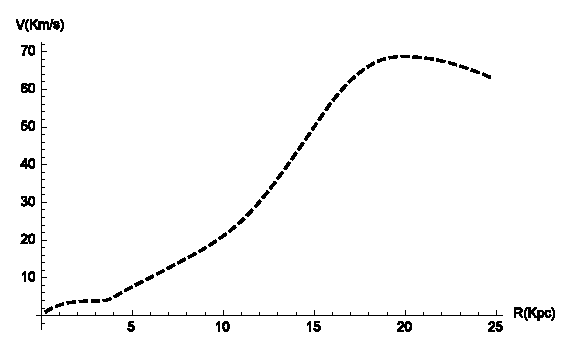
\includegraphics{Teste_gr1.eps}

\section*{Definindo Equa{\c c}{\~ o}es}

\begin{doublespace}
\noindent\(\pmb{\text{Vd}[\text{r$\_$},\text{M$\_$}]\text{:=}\frac{1}{2 \text{Rd}}\left(G \left(M *10^9\right) \left(\frac{r}{\text{Rd}}\right)^2\right) \left(\text{BesselI}\left[0,\frac{r}{2 \text{Rd}}\right] \text{BesselK}\left[0,\frac{r}{2 \text{Rd}}\right]-\text{BesselI}\left[1,\frac{r}{2 \text{Rd}}\right] \text{BesselK}\left[1,\frac{r}{2 \text{Rd}}\right]\right);}\\
\pmb{\text{Vme}[\text{r$\_$},\text{R$\_$},\text{P$\_$}]\text{:=}\frac{1}{r}6.4 G \left(\left(P *10^7\right) R^3\right) \left(\frac{1}{2} \text{Log}\left[\left(\frac{r}{R}\right)^2+1\right]+\text{Log}\left[\frac{r}{R}+1\right]-\text{ArcTan}\left[\frac{r}{R}\right]\right);}\\
\pmb{G\text{:=}\frac{4.302}{10^6};}\\
\pmb{\text{Rd}\text{:=}3.3;}\\
\pmb{\text{Vt}[\text{r$\_$},\text{M$\_$},\text{R$\_$},\text{P$\_$}]\text{:=}\text{Sqrt}[\text{Vd}[r,M]+\text{Vme}[r,R,P]+\text{Igas}[r]{}^{\wedge}2]}\)
\end{doublespace}

\begin{doublespace}
\noindent\(\pmb{\text{}}\)
\end{doublespace}

\section*{Ajuste }

\begin{doublespace}
\noindent\(\pmb{\text{Ajuste}= \text{NonlinearModelFit}[\text{RC},\text{Vt}[r,M,R,P],\{\{R,1,50\},\{M,1,30\},\{P,4,10\}\},r, \text{Weights}\to 1/\text{Erro}{}^{\wedge}2]}\)
\end{doublespace}

\begin{doublespace}
\noindent\(\text{FittedModel}\left[\right]\)
\end{doublespace}

\begin{doublespace}
\noindent\(\pmb{\text{Ajuste}[\text{{``}ParameterTable{''}}]}\)
\end{doublespace}

\begin{doublespace}
\noindent\(\begin{array}{l|llll}
 \text{} & \text{Estimate} & \text{Standard Error} & \text{t-Statistic} & \text{P-Value} \\
\hline
 R & 28.4899 & 5.9341 & 4.80105 & 0.0000764508 \\
 M & 45.5563 & 1.26035 & 36.1458 & \text{9.061970257549011$\grave{ }$*${}^{\wedge}$-22} \\
 P & 0.430196 & 0.0775027 & 5.55072 & 0.0000120272 \\
\end{array}\)
\end{doublespace}

\begin{doublespace}
\noindent\(\pmb{\text{}}\\
\pmb{a=\text{Plot}[\text{Ajuste}[x],\{x,0,24\},\text{AxesOrigin}\to \{0,0\}, \text{PlotStyle}\to \text{Black}];}\\
\pmb{\text{Show}[a,\text{ListPlot}[\text{RC}]];}\)
\end{doublespace}

